\documentclass[manuscript,screen,review]{acmart}
\citestyle{acmauthoryear}
\usepackage{booktabs}
\usepackage{multirow}
\usepackage{array}
\usepackage{graphicx}
\usepackage{amsmath}
\usepackage{tikz}
\usetikzlibrary{positioning,arrows.meta,fit,backgrounds}
\usepackage[ruled,vlined,linesnumbered]{algorithm2e}
\newcommand{\fit}[1]{\resizebox{\ifdim\width>\linewidth\linewidth\else\width\fi}{!}{#1}}
\setcopyright{acmlicensed}
\copyrightyear{2026}
\acmYear{2026}
\acmDOI{XXXXXXX.XXXXXXX}
\acmJournal{TALLIP}
\acmVolume{1}
\acmNumber{1}
\acmArticle{1}
\acmMonth{1}
\settopmatter{printacmref=true}

\begin{document}

\title[Do Hallucination Detectors Read the Context?]{Do Hallucination Detectors Read the Context? Transfer, Adaptation, and Grounding in Bengali Retrieval-Augmented Generation}

\author{Akib Hasan Pyil}
\email{23-50531-1@student.aiub.edu}
\affiliation{%
  \institution{American International University-Bangladesh (AIUB)}
  \department{Department of Computer Science}
  \city{Dhaka}
  \country{Bangladesh}
}

\author{Nazat E Rose Rhythm}
\email{23-50559-1@student.aiub.edu}
\affiliation{%
  \institution{American International University-Bangladesh (AIUB)}
  \department{Department of Computer Science}
  \city{Dhaka}
  \country{Bangladesh}
}

\author{Most. Sumaiya Habiba Nishat}
\email{23-50515-1@student.aiub.edu}
\affiliation{%
  \institution{American International University-Bangladesh (AIUB)}
  \department{Department of Computer Science}
  \city{Dhaka}
  \country{Bangladesh}
}

\author{Md. Ariful Islam}
\email{ariful@aiub.edu}
\affiliation{%
  \institution{American International University-Bangladesh (AIUB)}
  \department{Department of Computer Science}
  \city{Dhaka}
  \country{Bangladesh}
}

\author{S M Abdullah Shafi}
\email{shafi@aiub.edu}
\affiliation{%
  \institution{American International University-Bangladesh (AIUB)}
  \department{Department of Computer Science}
  \city{Dhaka}
  \country{Bangladesh}
}

\renewcommand{\shortauthors}{Pyil et al.}

\begin{abstract}
Hallucination detectors for retrieval-augmented generation are developed mostly in English, and their behaviour on low-resource languages is unclear. We compare seven detectors on the Bengali BangHallu benchmark under one protocol on a single 8~GB GPU. Two released LettuceDetect checkpoints, trained on English and Chinese data, lose about 0.24 Macro-F1 when moved to Bengali and fall below a lexical-overlap baseline, even on rows with a context passage; their tokenizers split a Bengali word into about eight to nine subwords. A Bengali-pretrained encoder, BanglaBERT-large, recovers most of this gap with a few hundred labelled examples and reaches 0.832 Macro-F1 with the full training set. An XLM-R sequence classifier did not train under five recipes, whereas the same backbone with a token-level multiple-instance head did. A post hoc analysis shows that on the 41.5\% of test rows without context the best detector is indistinguishable from a model that sees only the question and the answer, whereas on rows with context it reaches 0.921. Performance is lower on an external Bengali set and on a synthetic legal stress test. The study is empirical: a Bengali-pretrained encoder with a few hundred labelled examples is a workable starting point, and results should be reported separately for rows with and without evidence.
\end{abstract}

\begin{CCSXML}
<ccs2012>
   <concept>
       <concept_id>10010147.10010178.10010179</concept_id>
       <concept_desc>Computing methodologies~Natural language processing</concept_desc>
       <concept_significance>500</concept_significance>
       </concept>
   <concept>
       <concept_id>10010147.10010178.10010179.10010186</concept_id>
       <concept_desc>Computing methodologies~Language resources</concept_desc>
       <concept_significance>300</concept_significance>
       </concept>
   <concept>
       <concept_id>10002951.10003317.10003347.10003348</concept_id>
       <concept_desc>Information systems~Question answering</concept_desc>
       <concept_significance>300</concept_significance>
       </concept>
   <concept>
       <concept_id>10010147.10010257</concept_id>
       <concept_desc>Computing methodologies~Machine learning</concept_desc>
       <concept_significance>300</concept_significance>
       </concept>
 </ccs2012>
\end{CCSXML}

\ccsdesc[500]{Computing methodologies~Natural language processing}
\ccsdesc[300]{Computing methodologies~Language resources}
\ccsdesc[300]{Information systems~Question answering}
\ccsdesc[300]{Computing methodologies~Machine learning}

\keywords{hallucination detection, grounding, retrieval-augmented generation, Bengali, low-resource languages, cross-lingual transfer, calibration, tokenization}

\maketitle

\section{Introduction}
Retrieval-augmented generation (RAG) \cite{lewis2020rag} grounds a language model in documents it was not trained on, but grounding does not make the output faithful: generated answers still contradict, embellish, or ignore the retrieved passages \cite{ji2023survey,huang2025survey}. A common safeguard is a separate detector that reads the question, the retrieved context and the answer and flags unsupported content. Efficient encoder-based detectors of this kind, such as LettuceDetect \cite{kovacs2025lettucedetect}, are trained on RAGTruth \cite{niu2024ragtruth}, an English corpus, and are evaluated in English.

Bengali is widely spoken yet low-resource in the NLP literature \cite{bhattacharjee2022banglabert}, and it exposes three practical obstacles to reusing such detectors. The subword vocabularies of recent English-centric and European encoders fragment Bengali words; labelled data for hallucination detection is scarce; and the benchmark that does exist mixes two kinds of rows. BangHallu \cite{banghalluRepo} pairs Bengali questions with a correct and a constructed incorrect answer, and about four in ten of its rows carry no context passage. Its authors already treat rows with and without a passage as separate conditions in their own evaluation, but how detectors built to check answers against evidence behave on each side of that split has not been measured. Work on other lower-resource languages shows that detection quality drops with resource level \cite{ralethe2026multihallsa,abdaljalil2026halluverse} and that detectors transfer poorly across languages without in-language supervision \cite{datta2026lowresource}; Turk-LettuceDetect \cite{tas2025turk} adapts the LettuceDetect recipe to Turkish. For Bengali, we are not aware of a study that evaluates released RAG detectors zero-shot, traces how much Bengali supervision replaces them, and tests, by ablating the detector's input, whether the resulting detector uses the context it is given.

We ask five research questions:
\begin{itemize}
\item[\textbf{RQ1:}] Do released English and Chinese detectors transfer to Bengali without adaptation?
\item[\textbf{RQ2:}] How much Bengali supervision is needed, and does the choice of encoder and training formulation matter?
\item[\textbf{RQ3:}] What does a fine-tuned detector use on BangHallu rows with and without a context passage?
\item[\textbf{RQ4:}] Do the results hold on an external Bengali set and under a shift to the legal domain?
\item[\textbf{RQ5:}] Are the detectors calibrated, and what do they cost?
\end{itemize}

The two released detectors score below a lexical-overlap baseline, and neither truncation nor missing evidence explains the failure. BanglaBERT-large \cite{bhattacharjee2022banglabert} with its Bengali normalizer reaches 0.775 Macro-F1 with 564 examples. An XLM-R sequence classifier \cite{conneau2020xlmr} did not train under five recipes, while the same backbone with a token-level multiple-instance head reaches 0.730, so the failure is specific to the classification formulation in our setup. In a post hoc analysis, the best detector is indistinguishable from a question-and-answer-only model on the 41.5\% of test rows without context, which suggests that there it behaves like a plausibility classifier rather than a detector that checks evidence. The external and legal results are weaker than the in-domain ones, and we report them with their uncertainty.

\paragraph{Contributions.}
\begin{enumerate}
\item A controlled comparison of seven detectors (M0--M6) for Bengali under one protocol on a single 8~GB GPU, with seed-level variance, paired bootstrap intervals and Holm-corrected tests (Sections~\ref{sec:method}--\ref{sec:results}).
\item A tokenizer-fertility audit and a low-resource adaptation curve from zero to 5,627 Bengali examples, together with a fully documented negative result on XLM-R sequence classification (Sections~\ref{sec:fertility}--\ref{sec:adapt}).
\item A post hoc grounding analysis that splits BangHallu test rows by context availability and ablates the input of the best detector, showing what the detector uses on each subset (Section~\ref{sec:context}).
\item An external evaluation on Olikbochon with a leakage filter, a legal-domain stress test with gold and retrieved evidence, calibration and cost measurements, and an error analysis whose rule-based tagger we validate against LLM-drafted, author-reviewed labels and then correct for (Sections~\ref{sec:olik}--\ref{sec:errors}).
\item Code, frozen thresholds and per-example predictions that reproduce every number in the paper (Data and Code Availability).
\end{enumerate}

Section~\ref{sec:related} reviews related work, Section~\ref{sec:data} introduces Bengali and defines the task and data, Section~\ref{sec:method} describes the detectors and the evaluation protocol, Section~\ref{sec:results} reports results by research question, Section~\ref{sec:discussion} discusses them, Section~\ref{sec:validity} sets out the limitations, Section~\ref{sec:ethics} discusses ethical considerations, and Section~\ref{sec:conclusion} concludes.

\section{Related Work}\label{sec:related}
\paragraph{Hallucination and its detection.}
Surveys organise hallucination in generation into intrinsic and extrinsic types and review mitigation and detection \cite{ji2023survey,huang2025survey,maynez2020faithfulness}. For RAG, RAGTruth supplies word-level annotations of hallucinated spans in model responses \cite{niu2024ragtruth}, and LettuceDetect trains a ModernBERT \cite{warner2024modernbert} token classifier on it that is small and fast enough for production use \cite{kovacs2025lettucedetect}. QA-based metrics such as QAFactEval \cite{fabbri2022qafacteval} take a pipeline-style approach to factual consistency, and \citet{yang2026synonym} observe that detectors can flag a synonym of the correct token as a hallucination and add a synonym knowledge graph to counter this. These detectors are developed and evaluated in English; we use the released LettuceDetect checkpoints as our starting point and evaluate them at the answer level, the granularity that Bengali benchmarks provide.

\paragraph{Lower-resource and multilingual detection.}
Multi-Hall-SA reports that four state-of-the-art models detect up to 23.6\% fewer hallucinations in four South African languages than in English \cite{ralethe2026multihallsa}, and Halluverse-M$^3$ finds the lowest detection accuracy for Hindi among four languages \cite{abdaljalil2026halluverse}. \citet{datta2026lowresource} find detectors robust within a language but not across languages without in-language supervision, and Turk-LettuceDetect \cite{tas2025turk} adapts the LettuceDetect recipe to Turkish. Work on other low-resource tasks points the same way: \citet{munaf2024lowresource} adapt multilingual transformers to Urdu summarization by building an in-language dataset, \citet{lora2025conversum} address cross-lingual summarization when high-quality parallel data are scarce, and \citet{ahmat2023wadx} improve zero-shot cross-lingual transfer of multilingual encoders by aligning word representations with adapters. These studies establish that resource level matters; they do not ask whether a detector that scores well in a lower-resource language uses the evidence it is given. Our study adds a zero-shot test of released detectors, an adaptation curve from zero to full supervision, and an input ablation of the adapted detector.

\paragraph{Bengali hallucination resources.}
BangHallu was released with a project report by its authors \cite{banghalluRepo}. Its question--answer pairs were constructed with LLM assistance from Bengali Wikipedia passages and from school and civil-service question banks, and its labels were checked by human annotators. The report evaluates a ladder of systems up to fine-tuned BanglaBERT, reports rows with and without a passage separately, and defines a hard subset on which string matching fails. BenHalluEval \cite{adib2026benhallueval} evaluates large language models as hallucination detectors on Bengali across question answering, code-mixed question answering, summarization and reasoning. Neither evaluates released RAG detectors or tests, by input ablation, what a detector relies on when no passage is present; that is the gap our grounding analysis addresses.

\paragraph{Encoders, tokenization and Bengali.}
Multilingual encoders transfer unevenly across languages \cite{pires2019multilingual,conneau2020xlmr}, and a language's share of the subword vocabulary affects downstream quality \cite{rust2021tokenizer} and cost \cite{petrov2023tokenizer}. Studies of individual languages agree: for Turkish, the granularity and vocabulary size of the tokenizer change downstream performance \cite{toraman2023tokenization}; for Thai, missing foreign vocabulary in the tokenizer limits a pretrained model until the vocabulary is expanded \cite{sriwirote2025phayathaibert}; and for Bangla authorship attribution, word, subword and character tokenization give different results under transfer learning \cite{khatun2022authorship}. BanglaBERT \cite{bhattacharjee2022banglabert} is a Bengali-specific encoder released with a text normalizer. EuroBERT \cite{boizard2025eurobert} extends the modern encoder recipe to multiple languages, and ModernBERT \cite{warner2024modernbert} targets long context in English. We measure fertility for these four tokenizers on Bengali text and relate it to detection quality, without claiming a causal link.

\paragraph{Legal RAG.}
Legal retrieval-augmented systems still hallucinate at non-trivial rates \cite{magesh2025hallucination,das2026legalrag}, and citation-level auditing pipelines have been proposed for Brazilian Portuguese \cite{figueiredo2026grounded}. In lower-resource legal settings, general-purpose LLMs produce hallucinated answers to domain-specific Vietnamese legal questions \cite{le2025vietlegal}, MILPaC provides a benchmark for translating legal text into Indian languages \cite{mahapatra2025milpac}, and the divergence between auxiliary and target domains affects how well multilingual models adapt to low-resource translation \cite{ranathunga2026domain}. We do not build a legal system; we use two Bangladeshi legal question-answering resources \cite{banglagovragRepo,bdlegalqaRepo} to test whether a detector trained on general Bengali text survives a domain shift.

\section{Problem Formulation and Data}\label{sec:data}
\subsection{Bengali}\label{sec:bengali}
Bengali (Bangla) is the sixth most spoken language in the world, with over 300 million native speakers, yet it is considered resource-scarce for NLP \cite{bhattacharjee2022banglabert}: \citet{joshi2020state} place it among the languages that lack labelled data and rely on self-supervised pretraining. It is written in its own Brahmic script and has its own digits, which appear alongside Western digits in text. It is morphologically rich, and several of its characters have more than one Unicode representation; the text normalizer we use with BanglaBERT \cite{bhattacharjee2022banglabert} implements the normalization that \citet{hasan2020notlowresource} introduced to unify such characters. Three of these properties matter for this study. Tokenizers built mainly for English or European languages split Bengali words into many subword pieces (Section~\ref{sec:fertility}). Spelling, Unicode and digit variants make a surface comparison between an answer and its evidence brittle, which is why our error taxonomy has script-mismatch and digit-variant categories (Section~\ref{sec:errors}). And only a few labelled Bengali hallucination datasets exist (Section~\ref{sec:related}).

\subsection{Task definition}\label{sec:task}
Given a question $q$, a context passage $c$ (the evidence; possibly empty, $c=\emptyset$) and an answer $a$, a detector outputs a score $s(q,c,a)\in[0,1]$ for the answer being hallucinated, and a binary prediction $\hat{y}=\mathbb{1}[s(q,c,a)\geq\tau^*]$ for a threshold $\tau^*$. We use $y=1$ for an answer that is hallucinated, i.e.\ not supported by the context or factually incorrect, and invert sources that use the opposite convention (BangHallu marks faithful answers with 1). For a test set $T$ we write $T_{c}=\{(q,c,a)\in T: c\neq\emptyset\}$ and $T_{\emptyset}=T\setminus T_{c}$. On $T_{\emptyset}$ the label can only reflect factual correctness; this distinction is central to Section~\ref{sec:context}. Token-level detectors output a probability per answer token; we obtain an answer-level score by max pooling over answer tokens. Replacing max with the mean of the top three or top five token probabilities changes Macro-F1 by at most 0.009 for the models where it applies (M1, M2, M5).

\subsection{Datasets}\label{sec:datasets}
Table~\ref{tab:datasets} summarises the data. \textbf{BangHallu} \cite{banghalluRepo} is our main Bengali benchmark and is labelled at the answer level. According to its authors, the passages come from Bengali Wikipedia, the rows without a passage come mainly from school and civil-service exam question banks, and each question is paired with one correct and one incorrect answer, both constructed with LLM assistance from the source text and then checked by human annotators. Its splits are question-disjoint: no test or dev question occurs in the training split (2,924, 619 and 614 unique questions in train, dev and test). \textbf{Olikbochon} \cite{olikbochonKaggle} is the labelled sample of a Kaggle Bengali hallucination competition whose test file is unlabelled; we use its 299 labelled rows only for external evaluation. \textbf{RAGTruth} \cite{niu2024ragtruth} is the English source domain of the first released detector, and its Chinese translation (2,700 test examples) is the source domain of the second. For the legal domain we use \textbf{BanglaGovRAG} \cite{banglagovragRepo} and \textbf{BD Legal QA} \cite{bdlegalqaRepo}, which provide questions and reference answers but no hallucination labels (Section~\ref{sec:legal}). All Bengali sets were downloaded from their public repositories in October 2026; we did not record commit hashes, and the BD Legal QA repository has been updated since, so Table~\ref{tab:datasets} gives the row counts of the versions we used.

\begin{table}[t]
\caption{Datasets. ``Ctx.'' is the share of rows with a non-empty context passage. For Olikbochon and the legal sets the columns give the source splits; we train on none of them, and all their rows are used for evaluation only. Legal sets carry no hallucination labels; their detection task is constructed in Section~\ref{sec:legal}.}
\label{tab:datasets}
\small
\fit{\begin{tabular}{@{}lrrrrllp{3.1cm}@{}}
\toprule
Dataset & Train & Dev & Test & Ctx.\ (\%) & Labels & Halluc.\ (\%) & Role \\
\midrule
RAGTruth (English) & 14,942 & 0 & 2,675 & 100.0 & token/span + answer & 43.4 & source domain (released detectors) \\
BangHallu & 5,627 & 1,238 & 1,228 & 59.0 & answer-level & 50.0 & Bengali train / dev / test \\
Olikbochon & 239 & 29 & 31 & 43.5 & answer-level & 45.5 & external Bengali evaluation \\
BanglaGovRAG & 80 & 10 & 10 & 100.0 & reference answers only & -- & legal domain shift \\
BD Legal QA & 1,187 & 158 & 162 & 100.0 & reference answers only & -- & legal domain shift \\
\bottomrule
\end{tabular}}
\end{table}

\paragraph{Leakage control.}
We compared BangHallu train and test with an exact-match key on the (context, answer) pair and with character 4--5-gram TF-IDF cosine similarity between answers ($\geq 0.92$ with the same question, or $\geq 0.98$ regardless). The screen flagged 151 exact duplicates and 275 near-duplicate test rows. We left the test set untouched and removed every training row involved in a match: 507 rows, more than the flagged test rows because one test row can match several training rows. The training split shrank from 6,134 to 5,627 examples, and no model is trained on a row that duplicates a test row. Olikbochon is evaluated in full, but a later check found 30 rows (9 of them exact duplicates) with a counterpart in the cleaned training set; we report Olikbochon with and without them. The two legal sets showed no overlap.

\section{Detectors and Evaluation Protocol}\label{sec:method}
\subsection{Detectors}
Table~\ref{tab:models} lists the seven detectors. \textbf{M0} is a lexical containment baseline: the answer-level score is one minus the mean support of the answer's words, where a word counts as supported if it occurs in the context or its character trigrams are covered by the context. It needs no training and ignores the question. \textbf{M1} and \textbf{M2} are released LettuceDetect checkpoints used without any weight update: a ModernBERT-base token classifier trained on English RAGTruth, and a 210M-parameter EuroBERT token classifier trained on the Chinese translation of RAGTruth. Both are evaluated at their native 4,096-token limit with pinned model revisions. \textbf{M3} is XLM-R-base \cite{conneau2020xlmr} with a sequence-classification head trained with cross-entropy on BangHallu. \textbf{M4} is BanglaBERT-large \cite{bhattacharjee2022banglabert} with its text normalizer and a sequence-classification head. \textbf{M5} is XLM-R-base with a token-classification head trained with a multiple-instance-learning (MIL) loss: because BangHallu is labelled at the answer level, the maximum token probability over the answer is trained against the answer label. \textbf{M6} is Qwen2.5-3B-Instruct \cite{qwen2025qwen25} quantized to 4-bit NF4 \cite{dettmers2023qlora} and prompted zero-shot to say whether the answer is supported by the context; its score is the probability of the ``not supported'' reply normalized over the two replies. M6 is evaluated on a class-stratified subset of 600 test examples, with its threshold tuned on a stratified development subset of 300 examples. All fine-tuned models share the input layout (question, context, answer) and truncate the context, never the answer.

\begin{table}[t]
\caption{Detectors. ``Released'' models are used without any weight update; ``BH'' is the cleaned BangHallu training split. M5, not M3, is the XLM-R reference in the analyses (Section~\ref{sec:adapt}).}
\label{tab:models}
\small
\fit{\begin{tabular}{@{}l>{\raggedright}p{2.3cm}>{\raggedright}p{2.8cm}>{\raggedright}p{2.3cm}>{\raggedright}p{1.7cm}>{\raggedright\arraybackslash}p{1.9cm}@{}}
\toprule
ID & Backbone & Head / scoring & Training data & Bengali labels used & Role \tabularnewline
\midrule
M0 & -- (rule) & lexical containment of answer in context & none & dev threshold only & lexical baseline \tabularnewline
M1 & ModernBERT-base & token classifier, max pooling & English RAGTruth (released) & dev threshold only & released detector \tabularnewline
M2 & EuroBERT-210M & token classifier, max pooling & Chinese RAGTruth (released) & dev threshold only & released detector \tabularnewline
M3 & XLM-R-base & sequence classifier, cross-entropy & BH 0/10/25/100\% & train + dev & multilingual sequence model \tabularnewline
M4 & BanglaBERT-large + normalizer & sequence classifier, cross-entropy & BH 0/10/25/100\% & train + dev & Bengali encoder \tabularnewline
M5 & XLM-R-base & token classifier, MIL loss & BH 100\% & train + dev & multilingual token model \tabularnewline
M6 & Qwen2.5-3B-Instruct, 4-bit & zero-shot prompt, $p(\text{not supported})$ & none & dev threshold only & LLM verifier \tabularnewline
\bottomrule
\end{tabular}
}
\end{table}

\subsection{Evaluation protocol}
Figure~\ref{fig:pipeline} shows the stages of the study and Algorithm~\ref{alg:protocol} the scoring protocol shared by all detectors. For every detector, including the released ones, $\tau^*$ is tuned once on the BangHallu development set to maximize Macro-F1 and then frozen for the BangHallu test set and for all external and legal sets. For M1 and M2 this is the only use of Bengali labels; it can only favour them over an untuned threshold. Table~\ref{tab:design} maps each research question to its data, models, metrics and tests.

\begin{figure}[t]
\centering
\fit{% Study-design overview (Fig. 1). Diagram only: every count repeats a value stated in the text.
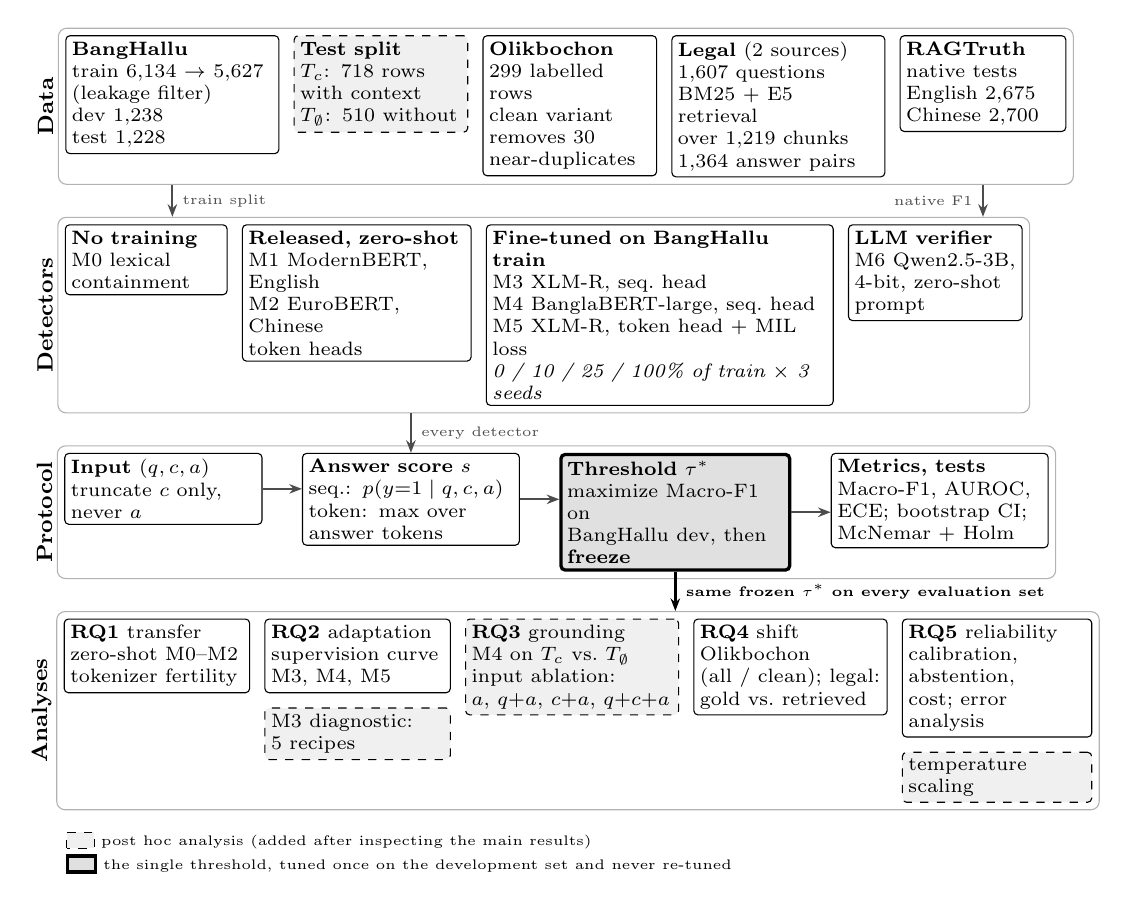
\begin{tikzpicture}[
  font=\scriptsize,
  >={Stealth[length=1.6mm]},
  box/.style={draw, rounded corners=1.5pt, align=left, inner sep=2.2pt, text width=#1, fill=white, anchor=north west, execute at begin node={\hyphenpenalty=10000\exhyphenpenalty=10000}},
  ph/.style={box=#1, dashed, fill=black!6},
  key/.style={box=#1, very thick, fill=black!12},
  head/.style={font=\footnotesize\bfseries, rotate=90, anchor=south, inner sep=1.5pt},
  grp/.style={draw=black!30, rounded corners=3pt, inner sep=2.5pt},
  flow/.style={->, thick, black!70},
  frz/.style={->, line width=1.2pt},
]
\def\g{1.8mm}
% ================= (1) DATA =================
\node[box=2.55cm] (bh) at (0,0) {\textbf{BangHallu}\\train 6,134 $\to$ 5,627\\(leakage filter)\\dev 1,238\\test 1,228};
\node[ph=2.05cm] (split) at ([xshift=\g]bh.north east) {\textbf{Test split}\\$T_c$: 718 rows\\with context\\$T_\emptyset$: 510 without};
\node[box=2.05cm] (olik) at ([xshift=\g]split.north east) {\textbf{Olikbochon}\\299 labelled rows\\clean variant\\removes 30\\near-duplicates};
\node[box=2.55cm] (legal) at ([xshift=\g]olik.north east) {\textbf{Legal} (2 sources)\\1,607 questions\\BM25 + E5 retrieval\\over 1,219 chunks\\1,364 answer pairs};
\node[box=1.95cm] (rt) at ([xshift=\g]legal.north east) {\textbf{RAGTruth}\\native tests\\English 2,675\\Chinese 2,700};
\begin{scope}[on background layer]\node[grp, fit=(bh)(split)(olik)(legal)(rt)] (gA) {};\end{scope}

% ================= (2) DETECTORS =================
\node[box=1.9cm] (m0) at ([xshift=2.5pt,yshift=-5mm]gA.south west) {\textbf{No training}\\M0 lexical\\containment};
\node[box=2.75cm] (rel) at ([xshift=\g]m0.north east) {\textbf{Released, zero-shot}\\M1 ModernBERT, English\\M2 EuroBERT, Chinese\\token heads};
\node[box=4.25cm] (ft) at ([xshift=\g]rel.north east) {\textbf{Fine-tuned on BangHallu train}\\M3 XLM-R, seq.\ head\\M4 BanglaBERT-large, seq.\ head\\M5 XLM-R, token head + MIL loss\\\textit{0 / 10 / 25 / 100\% of train $\times$ 3 seeds}};
\node[box=2.05cm] (m6) at ([xshift=\g]ft.north east) {\textbf{LLM verifier}\\M6 Qwen2.5-3B,\\4-bit, zero-shot\\prompt};
\begin{scope}[on background layer]\node[grp, fit=(m0)(rel)(ft)(m6)] (gB) {};\end{scope}

% ================= (3) PROTOCOL =================
\node[box=2.35cm] (inp) at ([xshift=2.5pt,yshift=-5mm]gB.south west) {\textbf{Input} $(q,c,a)$\\truncate $c$ only,\\never $a$};
\node[box=2.6cm] (sc) at ([xshift=5mm]inp.north east) {\textbf{Answer score} $s$\\seq.: $p(y{=}1\mid q,c,a)$\\token: max over\\answer tokens};
\node[key=2.75cm] (tau) at ([xshift=5mm]sc.north east) {\textbf{Threshold} $\tau^*$\\maximize Macro-F1 on\\BangHallu dev, then \textbf{freeze}};
\node[box=2.6cm] (met) at ([xshift=5mm]tau.north east) {\textbf{Metrics, tests}\\Macro-F1, AUROC,\\ECE; bootstrap CI;\\McNemar + Holm};
\draw[flow] (inp.east) -- (inp.east -| sc.west);
\draw[flow] (sc.east) -- (sc.east -| tau.west);
\draw[flow] (tau.east) -- (tau.east -| met.west);
\begin{scope}[on background layer]\node[grp, fit=(inp)(sc)(tau)(met)] (gC) {};\end{scope}

% ================= (4) ANALYSES =================
\node[box=2.2cm] (r1) at ([xshift=2.5pt,yshift=-5mm]gC.south west) {\textbf{RQ1} transfer\\zero-shot M0--M2\\tokenizer fertility};
\node[box=2.2cm] (r2) at ([xshift=\g]r1.north east) {\textbf{RQ2} adaptation\\supervision curve\\M3, M4, M5};
\node[ph=2.55cm] (r3) at ([xshift=\g]r2.north east) {\textbf{RQ3} grounding\\M4 on $T_c$ vs.\ $T_\emptyset$\\input ablation:\\$a$, $q{+}a$, $c{+}a$, $q{+}c{+}a$};
\node[box=2.3cm] (r4) at ([xshift=\g]r3.north east) {\textbf{RQ4} shift\\Olikbochon\\(all / clean); legal:\\gold vs.\ retrieved};
\node[box=2.25cm] (r5) at ([xshift=\g]r4.north east) {\textbf{RQ5} reliability\\calibration, abstention,\\cost; error analysis};
\node[ph=2.2cm] (r2b) at ([yshift=-\g]r2.south west) {M3 diagnostic:\\5 recipes};
\node[ph=2.25cm] (r5b) at ([yshift=-\g]r5.south west) {temperature scaling};
\begin{scope}[on background layer]\node[grp, fit=(r1)(r2)(r3)(r4)(r5)(r2b)(r5b)] (gD) {};\end{scope}


% ================= band titles (left margin) =================
\node[head] at (gA.west) {Data};
\node[head] at (gB.west) {Detectors};
\node[head] at (gC.west) {Protocol};
\node[head] at (gD.west) {Analyses};

% ================= band-to-band flows =================
\draw[flow] (bh.south |- gA.south) -- node[right, font=\tiny]{train split} (bh.south |- gB.north);
\draw[flow] (rt.south |- gA.south) -- node[left, font=\tiny]{native F1} (rt.south |- gB.north);
\draw[flow] (sc.north |- gB.south) -- node[right, font=\tiny]{every detector} (sc.north);
\draw[frz] (tau.south) -- node[right, font=\tiny\bfseries]{same frozen $\tau^*$ on every evaluation set} (tau.south |- gD.north);

% ================= legend =================
\node[anchor=north west, align=left, font=\tiny] at ([yshift=-1.5mm]gD.south west) {%
\tikz[baseline=-0.6ex]\draw[dashed, fill=black!6] (0,-0.08) rectangle (0.35,0.12);~post hoc analysis (added after inspecting the main results)\\[1pt]
\tikz[baseline=-0.6ex]\draw[very thick, fill=black!12] (0,-0.08) rectangle (0.35,0.12);~the single threshold, tuned once on the development set and never re-tuned};
\end{tikzpicture}
}
\caption{Study design. (1)~Data with the leakage filter and the post hoc split of BangHallu test by context availability; (2)~seven detectors grouped by how much Bengali supervision they receive; (3)~the protocol shared by all detectors, in which one threshold tuned on the BangHallu development set is frozen; (4)~the analyses for each research question. Dashed boxes are post hoc analyses (Section~\ref{sec:posthoc}).}
\Description{Diagram with four horizontal bands, from top to bottom. Band 1, data: BangHallu with training rows reduced from 6,134 to 5,627 by a leakage filter, a development set of 1,238 and a test set of 1,228 rows that is split, post hoc, into 718 rows with a context passage and 510 without; Olikbochon with 299 labelled rows; a legal set of 1,607 questions with retrieval over 1,219 chunks and 1,364 reference-versus-perturbation pairs; and the RAGTruth native English and Chinese test sets. Band 2, detectors: a lexical baseline with no training; two released zero-shot token detectors; three detectors fine-tuned on BangHallu with 0, 10, 25 or 100 percent of the training data and three seeds; and a 4-bit LLM verifier. Band 3, shared protocol: input of question, context and answer with only the context truncated, a score per answer, a threshold tuned once on the development set and frozen, metrics, and statistical tests. A thick arrow labelled frozen threshold leads down to band 4, analyses: zero-shot transfer and tokenizer fertility; the supervision curve and a post hoc diagnostic of five recipes for the XLM-R sequence classifier; the post hoc context split and input ablation with four input variants; the external and legal evaluations; and calibration, selective prediction, cost and error analysis, with post hoc temperature scaling.}
\label{fig:pipeline}
\end{figure}

\begin{algorithm}[t]
\caption{Scoring and threshold protocol shared by all detectors}\label{alg:protocol}
\SetKwInOut{Input}{Input}\SetKwInOut{Output}{Output}
\Input{detector $f$; maximum input length $L$; BangHallu development set $D$; evaluation sets $\mathcal{T}$}
\Output{frozen threshold $\tau^*$; per-set metrics with bootstrap intervals}
\ForEach{example $(q,c,a)$ in $D$ and in every $T\in\mathcal{T}$}{
  build the input $(q,c,a)$; if it exceeds $L$ tokens, truncate $c$ only, never $a$\;
  \eIf{$f$ is a token-level detector}{$s \leftarrow \max_{t\in a} p_f(t)$ over answer tokens\;}{$s \leftarrow p_f(y=1\mid q,c,a)$\;}
}
$\tau^* \leftarrow \arg\max_\tau \text{Macro-F1}(D,\tau)$; freeze $\tau^*$\;
\ForEach{$T\in\mathcal{T}$}{
  $\hat{y}\leftarrow\mathbb{1}[s\geq\tau^*]$; compute Macro-F1, AUROC, AUPRC and ECE\;
  compute 95\% percentile intervals from 1,000 bootstrap resamples of the examples of $T$\;
  \textit{post hoc:} repeat the two previous lines on $T_c$ and $T_\emptyset$ separately\;
}
\end{algorithm}

\begin{table}[t]
\caption{Experimental design. Each research question with its data, detectors, primary metric and test. Post hoc analyses are marked.}
\label{tab:design}
\small
\fit{\begin{tabular}{@{}>{\raggedright}p{2.5cm}>{\raggedright}p{2.7cm}>{\raggedright}p{2.2cm}>{\raggedright}p{2.2cm}>{\raggedright\arraybackslash}p{2.9cm}@{}}
\toprule
RQ & Data & Detectors & Primary metric & Test / interval \tabularnewline
\midrule
RQ1 transfer & BangHallu test; native test sets & M0, M1, M2 & Macro-F1, AUROC & bootstrap CI; paired bootstrap + McNemar (Holm) \tabularnewline
RQ1 fertility & RAGTruth, BangHallu text & four tokenizers & tokens per word, truncation rate & descriptive \tabularnewline
RQ2 adaptation & BangHallu, 0/10/25/100\% of train & M3, M4, M5 & Macro-F1 (3 seeds) & bootstrap CI; paired bootstrap + McNemar (Holm) \tabularnewline
RQ2 M3 diagnostic (post hoc) & BangHallu & M3, five recipes & train loss, dev AUROC & descriptive \tabularnewline
RQ3 context split (post hoc) & BangHallu test, $T_c$ / $T_\emptyset$ & M0--M5 & Macro-F1 per subset & bootstrap CI; paired bootstrap contrasts \tabularnewline
RQ3 input ablation (post hoc) & BangHallu & M4 on reduced input & Macro-F1 per subset & paired bootstrap contrasts \tabularnewline
RQ4 external & Olikbochon (all / clean, post hoc) & M0, M1, M2, M4 & Macro-F1, AUROC & bootstrap CI; paired bootstrap \tabularnewline
RQ4 legal & BanglaGovRAG + BD Legal QA & M0--M4 & Macro-F1, recall, FAR & mean $\pm$ SD over seeds \tabularnewline
RQ5 calibration & BangHallu dev / test & M4, M5 (temperature scaling post hoc) & ECE, NLL, Brier, AURC & mean over seeds \tabularnewline
RQ5 cost & BangHallu test & M0--M6 & ms per example, peak memory & descriptive \tabularnewline
\bottomrule
\end{tabular}
}
\end{table}

\subsection{Training}
M3, M4 and M5 are trained with AdamW \cite{loshchilov2019adamw} (weight decay 0.01), a linear schedule with 10\% warm-up, gradient clipping at 1.0, an effective batch size of 16 by gradient accumulation, bf16 autocast and a maximum length of 512 tokens. M4 uses a learning rate of $1.5\times10^{-5}$ with 5, 8 and 10 epochs for 100\%, 25\% and 10\% of the training data; M5 uses $2\times10^{-5}$ and 5 epochs. The original M3 runs used $3\times10^{-5}$ and 8, 10 and 12 epochs without the normalizer. Early stopping monitors development AUROC with a patience of four epochs, so with five to twelve epochs it can stop a run only late in training. Each configuration is trained with three seeds (42, 1337, 2026), and the 10\% and 25\% subsets are sampled in question groups. Because of the 8~GB memory budget, the large word-embedding matrices of the XLM-R models are frozen, and the optimizer (fused or 8-bit AdamW \cite{dettmers2022optimizers}) is chosen by a memory estimate before each run. All experiments ran on a single consumer GPU (RTX~4060, 8~GB). Appendix~\ref{app:impl} collects these settings in one table.

\subsection{Metrics and statistics}
The primary metric is answer-level Macro-F1 (both classes weighted equally, so that chance is about 0.5, and predicting a single class gives 0.333). We also report AUROC, AUPRC, and expected calibration error \cite{guo2017calibration} (ECE, ten equal-width bins, top-label confidence). Means and standard deviations are over the three seeds; for single deterministic models (M0, M1, M2) we report the value without a standard deviation. Confidence intervals are 95\% percentile intervals from 1,000 bootstrap resamples of test examples, with seed-averaged F1 for multi-seed models. The four primary model comparisons are tested with paired bootstrap intervals \cite{bergkirkpatrick2012significance} and McNemar's test \cite{mcnemar1947note} on majority-vote predictions (a row is predicted positive if at least two of the three seed-level predictions, each at its own $\tau^*$, are positive), so the F1 values in the paired-comparison table are vote-F1 and differ from the seed-mean F1 reported elsewhere. Their $p$-values are Holm-adjusted \cite{holm1979sequential} over these four comparisons, and the effect size is Cohen's $h$ \cite{cohen1988power} between the two models' proportions of correct predictions; we follow \citet{dror2018hitchhiker} on choosing and reporting tests. All other intervals in the paper, including the contrasts of Section~\ref{sec:context}, are paired bootstrap intervals without multiplicity correction and are descriptive. Selective prediction is summarised by the area under the risk--coverage curve (AURC) \cite{geifman2017selective}, with confidence taken as the distance of the score from $\tau^*$.

\subsection{Analyses added after the main run}\label{sec:posthoc}
After inspecting the main results we added five analyses: a split of BangHallu test by context availability; an ablation of M4's input (three seeds per variant, same recipe); a diagnostic for the failed M3 runs; a leakage-filtered Olikbochon evaluation; and temperature scaling of the fine-tuned models. Only the ablation and the diagnostic train new models; the other three reuse the original predictions and thresholds. They are labelled as post hoc where they appear. Original thresholds, predictions and tables were verified to be unchanged by these analyses.

\section{Results}\label{sec:results}
\subsection{Zero-shot transfer fails (RQ1)}\label{sec:transfer}
Table~\ref{tab:transfer} compares the released detectors, M1 (English, ModernBERT) and M2 (Chinese, EuroBERT), on their native test sets and on BangHallu. Both lose about 0.24 Macro-F1 (M1: 0.773$\to$0.533; M2: 0.746$\to$0.508) and land close to chance, with AUROC of 0.546 and 0.512. Both fall below the lexical baseline M0 (0.653, 95\% CI $[0.624, 0.679]$), which uses no learning. The Chinese-trained EuroBERT detector is slightly worse than the English ModernBERT detector (paired $\Delta=-0.025$, CI $[-0.050, -0.000]$, McNemar $\chi^2(1)=6.3$, $p_\mathrm{Holm}=0.012$; Table~\ref{tab:sig}), so a closer source language does not help. Calibration is poor as well: the ECE of M1 and M2 is 0.446 and 0.301.

Input truncation does not explain the drop: at their native 4,096-token limit, 0.16\% (ModernBERT) and 0\% (EuroBERT) of BangHallu examples are truncated. Nor does missing evidence: restricting to rows that do contain a context passage raises M1 only to 0.575 and leaves M2 at 0.491 (Section~\ref{sec:context}), still 0.20 and 0.26 below the native scores.

\begin{figure}[t]
\centering
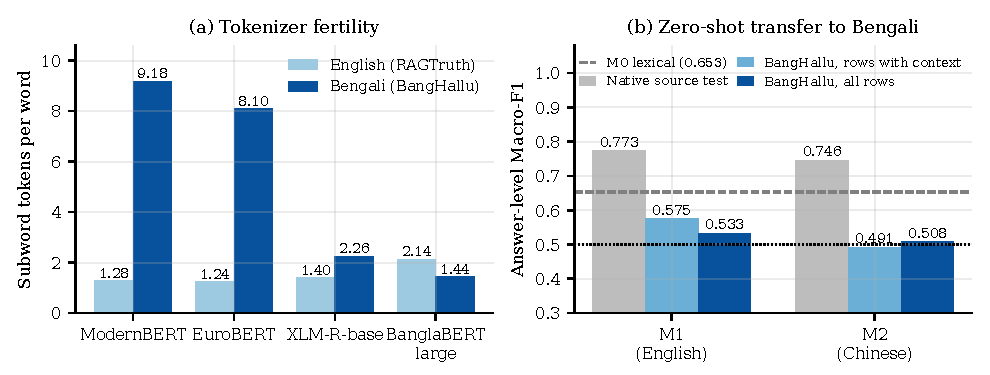
\includegraphics[width=\linewidth]{figures/fig_fertility_transfer.pdf}
\caption{Tokenizer fertility and zero-shot transfer. (a)~Subword tokens per word for the four tokenizers on English (RAGTruth) and Bengali (BangHallu) text: the two released detectors' tokenizers fragment Bengali words most. (b)~Answer-level Macro-F1 of the released detectors on their native test sets, on BangHallu rows that contain a context passage, and on all BangHallu rows: both stay below the lexical baseline (dashed line) even with context.}
\Description{Two-panel bar chart. Left: subword tokens per word for four tokenizers on English and Bengali text; ModernBERT and EuroBERT need about 9 and 8 tokens per Bengali word, XLM-R about 2.3 and BanglaBERT-large about 1.4. Right: Macro-F1 of the two released detectors on their native test sets (about 0.75) compared with BangHallu rows with context (0.575 and 0.491) and all BangHallu rows (about 0.5), with a dashed line for the lexical baseline at 0.65.}
\label{fig:fertility}
\end{figure}

\begin{table}[t]
\caption{Zero-shot transfer to BangHallu (1,228 test rows): both released detectors fall below the lexical baseline. ``Native F1'' is Macro-F1 on the source-language test set (RAGTruth English, 2,675 examples; Chinese translation, 2,700); $\Delta$ is BangHallu F1 minus native F1. M1 and M2 are single deterministic runs.}
\label{tab:transfer}
\small
\fit{\begin{tabular}{@{}lcccccc c@{}}
\toprule
Model & Native F1 & BH F1 & 95\% CI & AUROC & AUPRC & ECE & $\Delta$ \\
\midrule
M0 Lexical containment & -- & 0.653 & [0.624, 0.679] & 0.594 & 0.534 & 0.429 & -- \\
M1 LettuceDetect (ModernBERT, English) & 0.773 & 0.533 & [0.506, 0.562] & 0.546 & 0.527 & 0.446 & $-0.240$ \\
M2 LettuceDetect (EuroBERT-210M, Chinese) & 0.746 & 0.508 & [0.482, 0.536] & 0.512 & 0.514 & 0.301 & $-0.237$ \\
\bottomrule
\end{tabular}}
\end{table}

\subsection{Tokenizer fertility (RQ1)}\label{sec:fertility}
Figure~\ref{fig:fertility}a gives a plausible mechanism, though not a proof of one. The ModernBERT and EuroBERT vocabularies split a Bengali word into 9.18 and 8.10 subword tokens on average, against 1.28 and 1.24 for English, about a seven-fold inflation relative to English for the same tokenizer; XLM-R-base needs 2.26 tokens per word for Bengali and BanglaBERT-large 1.44. Fertility of this size makes a token-level detector classify fragments of words, and it makes Bengali inputs long: at a 512-token budget, 28.5\% (ModernBERT) and 24.4\% (EuroBERT) of Bengali examples would be truncated, and naive tail truncation would remove 2.06\% and 0.83\% of answer tokens. Our fine-tuned models avoid this: only 0.81\% (XLM-R) and 0.33\% (BanglaBERT) of Bengali examples exceed 512 tokens, and because only the context is truncated, no answer token is ever lost. We cannot separate fertility from the fact that neither backbone targets Bengali (ModernBERT is trained mainly on English text, EuroBERT on European and a set of widely spoken languages); no experiment here changes one while holding the other fixed. The contrast between M3, M4 and M5 below is the closest evidence we have.

\subsection{Adaptation with Bengali supervision (RQ2)}\label{sec:adapt}
Table~\ref{tab:adapt} and Figure~\ref{fig:adapt} show the supervision curve. The zero-supervision row is the freshly initialised classification head and serves only as a floor (about 0.50). BanglaBERT-large with the normalizer (M4) reaches 0.775 Macro-F1 with 564 training examples (10\%), 0.785 with 1,408 and 0.832 with all 5,627. The 10\% model retains 93\% of the full-data score; the remaining gap is small but significant ($-0.040$, CI $[-0.062,-0.019]$, $\chi^2(1)=11.9$, $p_\mathrm{Holm}=0.0011$, Table~\ref{tab:sig}). The paired comparisons in Table~\ref{tab:sig} use majority-vote predictions, which score higher than the seed means of Table~\ref{tab:adapt} (M4 at 100\%: 0.843 against 0.832; M4 at 10\%: 0.803 against 0.775; the XLM-R sequence classifier M3: 0.537 against 0.502). On that basis, at full supervision M4 outperforms the Chinese-trained released detector (M2) by 0.334 (CI $[0.301, 0.367]$) and the XLM-R sequence classifier by 0.306 (CI $[0.275, 0.339]$), with $\chi^2(1)=278.9$ and $251.1$, both $p_\mathrm{Holm}<10^{-55}$, and Cohen's $h$ of 0.73 and 0.68. The XLM-R token detector M5 reaches 0.730 $\pm$ 0.008, below M4 by 0.102 in seed-averaged F1 (CI $[0.080, 0.124]$) but well above M0.

\begin{figure}[t]
\centering
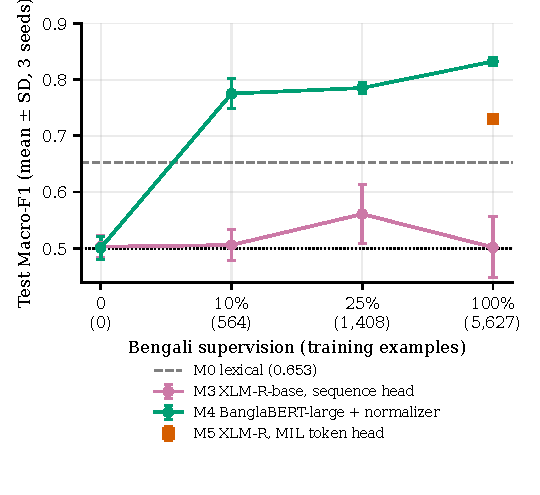
\includegraphics[width=0.62\linewidth]{figures/fig_adaptation.pdf}
\caption{Test Macro-F1 versus the amount of Bengali supervision (mean $\pm$ SD over three seeds). BanglaBERT-large passes the lexical baseline with 564 examples; the XLM-R sequence classifier does not leave chance level at any supervision level.}
\Description{Line chart of test Macro-F1 against the number of Bengali training examples. BanglaBERT-large rises from about 0.50 with no supervision to 0.775 at 564 examples and 0.832 at 5,627 examples. The XLM-R sequence classifier stays between 0.50 and 0.56. A single point for the XLM-R token detector is at 0.73 and a dashed line marks the lexical baseline at 0.65.}
\label{fig:adapt}
\end{figure}

\begin{table}[t]
\caption{Paired comparisons on BangHallu test. F1 values are Macro-F1 of majority-vote predictions (not seed means; see Table~\ref{tab:adapt}) and $\Delta$ is computed before rounding. $p$-values are McNemar $p$-values adjusted with the Holm procedure over the four comparisons.}
\label{tab:sig}
\small
\fit{\begin{tabular}{@{}lccccccc@{}}
\toprule
Comparison & F1 (A) & F1 (B) & $\Delta$ F1 & 95\% paired CI & McNemar $\chi^2(1)$ & $p$ (Holm) & Cohen's $h$ \\
\midrule
M2-CN vs M1-EN & 0.508 & 0.533 & $-0.025$ & [$-$0.050, $-$0.000] & 6.3 & 0.0119 & $-0.07$ \\
M4-100\% vs M2-CN & 0.843 & 0.508 & $+0.334$ & [0.301, 0.367] & 278.9 & $5.3\times10^{-62}$ & $+0.73$ \\
M4-100\% vs M3-100\% & 0.843 & 0.537 & $+0.306$ & [0.275, 0.339] & 251.1 & $4.4\times10^{-56}$ & $+0.68$ \\
M4-10\% vs M4-100\% & 0.803 & 0.843 & $-0.040$ & [$-$0.062, $-$0.019] & 11.9 & 0.0011 & $-0.10$ \\
\bottomrule
\end{tabular}}
\end{table}

\begin{table}[t]
\caption{Adaptation to Bengali with 0, 10, 25 and 100\% of the 5,627 training examples (three seeds; the 0\% rows are an untrained head): 564 examples already give BanglaBERT-large 93\% of its full-data Macro-F1. CI is a seed-averaged bootstrap interval.}
\label{tab:adapt}
\small
\fit{\begin{tabular}{@{}lrrcccc@{}}
\toprule
Model & \% & Examples & Macro-F1 & 95\% CI & AUROC & ECE \\
\midrule
M3 XLM-R-base (sequence head) & 0 & 0 & 0.503 $\pm$ 0.019 & [0.487, 0.516] & 0.504 $\pm$ 0.019 & 0.056 $\pm$ 0.043 \\
M3 XLM-R-base (sequence head) & 10 & 564 & 0.506 $\pm$ 0.027 & [0.489, 0.523] & 0.539 $\pm$ 0.021 & 0.013 $\pm$ 0.003 \\
M3 XLM-R-base (sequence head) & 25 & 1,408 & 0.561 $\pm$ 0.053 & [0.542, 0.580] & 0.585 $\pm$ 0.070 & 0.053 $\pm$ 0.020 \\
M3 XLM-R-base (sequence head) & 100 & 5,627 & 0.502 $\pm$ 0.054 & [0.484, 0.521] & 0.528 $\pm$ 0.018 & 0.015 $\pm$ 0.002 \\
\midrule
M4 BanglaBERT-large + normalizer & 0 & 0 & 0.501 $\pm$ 0.020 & [0.487, 0.514] & 0.510 $\pm$ 0.032 & 0.028 $\pm$ 0.029 \\
M4 BanglaBERT-large + normalizer & 10 & 564 & 0.775 $\pm$ 0.027 & [0.755, 0.794] & 0.853 $\pm$ 0.025 & 0.154 $\pm$ 0.050 \\
M4 BanglaBERT-large + normalizer & 25 & 1,408 & 0.785 $\pm$ 0.010 & [0.767, 0.803] & 0.892 $\pm$ 0.013 & 0.096 $\pm$ 0.015 \\
M4 BanglaBERT-large + normalizer & 100 & 5,627 & 0.832 $\pm$ 0.007 & [0.814, 0.850] & 0.933 $\pm$ 0.005 & 0.117 $\pm$ 0.007 \\
\midrule
M5 XLM-R-base (token head, MIL loss) & 100 & 5,627 & 0.730 $\pm$ 0.008 & -- & 0.837 & -- \\
\bottomrule
\end{tabular}}
\end{table}

\paragraph{The XLM-R sequence classifier did not train.}
M3 stays at 0.50--0.56 Macro-F1 at every supervision level (Table~\ref{tab:adapt}). Because a model that does not train cannot support any claim about the backbone, we investigated it before interpreting the comparison with M4 (post hoc). We trained XLM-R-base with a sequence head on the full training set with four additional recipes (learning rates $10^{-5}$, $2\times10^{-5}$ and $5\times10^{-5}$ without the normalizer, and $2\times10^{-5}$ with it), eight epochs, no early stopping and a fixed seed, next to the original run (Table~\ref{tab:m3diag}). In all five, the training loss stays at 0.695, essentially $\ln 2$, the best development AUROC is at most 0.542, the standard deviation of predicted probabilities on the development set is at most 0.004, and three of the five test predictions at the 0.5 threshold are a single class (Macro-F1 0.333). Figure~\ref{fig:dynamics} contrasts these runs with M5, which uses the same backbone, the same frozen embeddings and a similar learning rate but a token-level head with a MIL loss: its training loss falls from 0.70 to 0.41 and its development AUROC rises from 0.69 to 0.85 in five epochs. We did not find the cause. The comparison supports only a narrow conclusion: in our setup, with frozen embeddings and a classification head on the first token, XLM-R-base did not learn BangHallu, while the same backbone with a token-level head did. We therefore use M5, not M3, as the XLM-R reference in the rest of the paper, and we do not interpret M3 as evidence about multilingual encoders in general. Whether unfreezing the embeddings, which our memory budget did not allow us to test for all settings, would change this remains open.

\begin{table}[t]
\caption{Diagnostic runs for the XLM-R sequence classifier (post hoc; full training set, seed 42; the first row is the original configuration): no recipe moves the training loss away from $\ln 2$. Loss is the final training loss; dev-prob.\ SD is the standard deviation of predicted probabilities on the development set.}
\label{tab:m3diag}
\small
\fit{\begin{tabular}{@{}lrccccccc@{}}
\toprule
Setting & Ep. & Train loss & Dev AUROC & Dev-prob.\ SD & Test F1 ($\tau^*$) & Test F1 (0.5) & Test AUROC \\
\midrule
Original: lr 3e-5, normalizer off, early stop & 5 & 0.696 & 0.540 & -- & 0.541 & 0.333 & 0.546 \\
lr 1e-05, normalizer off & 8 & 0.695 & 0.532 & 0.001 & 0.522 & 0.489 & 0.531 \\
lr 2e-05, normalizer off & 8 & 0.695 & 0.542 & 0.004 & 0.545 & 0.333 & 0.551 \\
lr 5e-05, normalizer off & 8 & 0.695 & 0.517 & 0.000 & 0.490 & 0.333 & 0.495 \\
lr 2e-05, normalizer on & 8 & 0.695 & 0.520 & 0.002 & 0.518 & 0.414 & 0.516 \\
\bottomrule
\end{tabular}}
\end{table}

\begin{figure}[t]
\centering
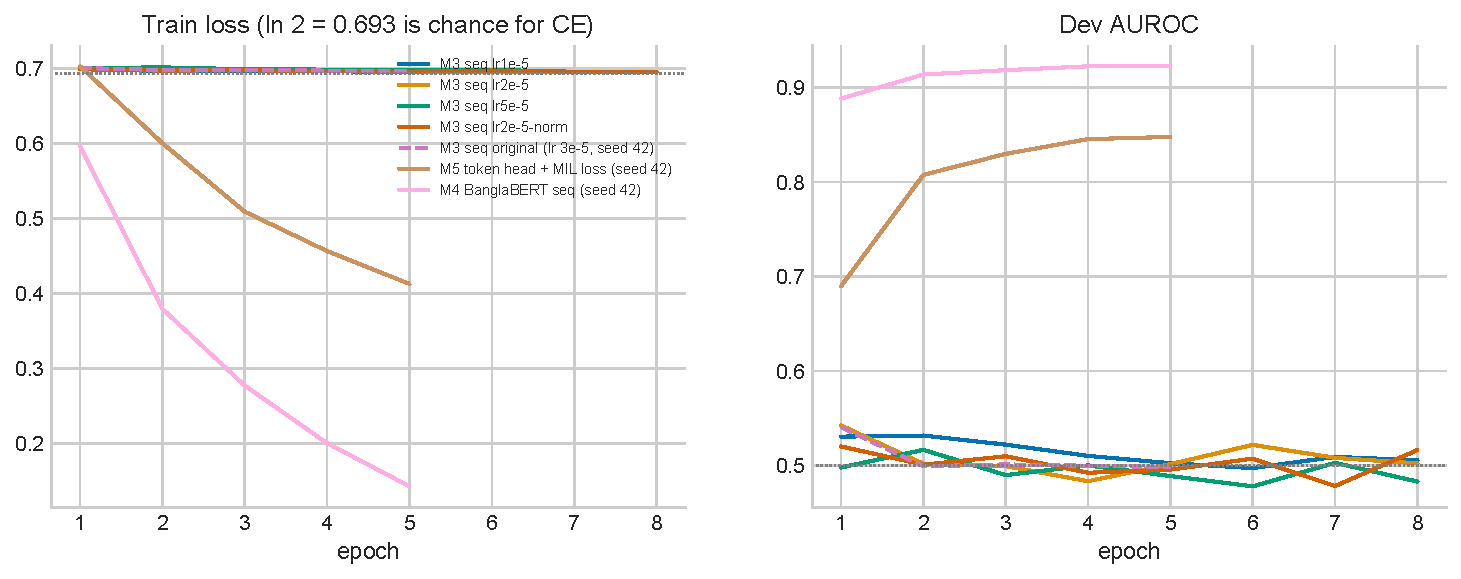
\includegraphics[width=\linewidth]{figures/fig_training_dynamics.pdf}
\caption{Training dynamics (seed 42): the five XLM-R sequence-classification runs stay at chance (loss $\approx\ln 2$, development AUROC $\approx0.5$), while the XLM-R token detector with a MIL loss (M5) and BanglaBERT-large (M4) train normally. The M3 runs lasted five or eight epochs; M5 and M4 five.}
\Description{Two line charts over training epochs. Left: training loss. Five XLM-R sequence-classification runs stay flat near 0.69, while the XLM-R token detector and BanglaBERT-large fall steadily. Right: development AUROC. The XLM-R sequence runs stay near 0.5, while the token detector rises to about 0.85 and BanglaBERT-large to about 0.92.}
\label{fig:dynamics}
\end{figure}

\subsection{What a fine-tuned detector uses with and without context (RQ3)}\label{sec:context}
Only 59\% of BangHallu rows have a context passage (Table~\ref{tab:datasets}). In the test set 718 rows (58.5\%) have one and 510 (41.5\%) do not. The BangHallu authors already report the two conditions separately for their own systems \cite{banghalluRepo}; our question is what the detectors in this study do on each subset. This split was not part of our original plan: we examined it after noticing that the lexical baseline flagged every answer token on a large share of rows, and we report it as a post hoc analysis. Table~\ref{tab:context} gives each model's Macro-F1 on the two subsets.

\begin{table}[t]
\caption{Macro-F1 on BangHallu test rows with and without a context passage (post hoc analysis): detectors that rely only on the context fall to a single class without it, while the fine-tuned models stay above chance. $\Delta$ is the with-context minus without-context F1 of the same model. Intervals are seed-averaged bootstrap intervals.}
\label{tab:context}
\small
\fit{\begin{tabular}{@{}lcccccc@{}}
\toprule
 & All & \multicolumn{2}{c}{With context ($n{=}718$)} & \multicolumn{2}{c}{Without context ($n{=}510$)} & $\Delta$ \\
\cmidrule(lr){3-4}\cmidrule(lr){5-6}
Model & F1 & F1 & 95\% CI & F1 & 95\% CI & \\
\midrule
M0 lexical containment & 0.653 & 0.779 & [0.745, 0.808] & 0.333 & [0.314, 0.353] & 0.446 \\
M1 released English & 0.533 & 0.575 & [0.539, 0.612] & 0.333 & [0.314, 0.353] & 0.242 \\
M2 released EuroBERT (Chinese) & 0.508 & 0.491 & [0.455, 0.526] & 0.390 & [0.354, 0.428] & 0.101 \\
M3 XLM-R seq.\ (collapsed) & 0.502 & 0.486 $\pm$ 0.029 & [0.463, 0.507] & 0.432 $\pm$ 0.066 & [0.404, 0.460] & 0.054 \\
M5 XLM-R, MIL token head & 0.730 & 0.854 $\pm$ 0.013 & [0.831, 0.877] & 0.552 $\pm$ 0.033 & [0.519, 0.582] & 0.302 \\
M4 BanglaBERT-large & 0.832 & 0.921 $\pm$ 0.006 & [0.902, 0.936] & 0.705 $\pm$ 0.015 & [0.672, 0.736] & 0.216 \\
\bottomrule
\end{tabular}}
\end{table}

On rows without context, the detectors that can only compare the answer with the context fail: the lexical baseline M0 predicts a single class there (Macro-F1 0.333), as does the released English detector M1 (0.333), and the Chinese-trained M2 reaches 0.390. The fine-tuned models do not fail in the same way; BanglaBERT-large (M4) reaches 0.705 and the XLM-R token detector (M5) 0.552 on the same rows. On rows with evidence, the gaps between the fine-tuned models and the baselines are wider than on the full test set. With context, M4 scores 0.921 (CI $[0.902, 0.936]$), M5 0.854, M0 0.779 and the released detectors 0.575 and 0.491. M4 exceeds M5 by 0.066 (CI $[0.046, 0.089]$) with context and by 0.153 (CI $[0.111, 0.193]$) without, so much of the overall gap between the two comes from the evidence-free rows. M4's error rate is 7.4\% with context and 29.8\% without, and 152 of its 205 errors (74\%) fall on rows without context.

\paragraph{Input ablation of M4.}
To see what M4 uses, we retrained it three times per variant with the same recipe on reduced input (post hoc; Table~\ref{tab:ground}, Figure~\ref{fig:context}). Using the answer alone gives 0.572 Macro-F1 (AUROC 0.618), above chance but weak. Adding the question gives 0.703 overall, and the result is the same on both subsets: 0.704 with context and 0.700 without. On the evidence-free rows the full model (0.705) is thus indistinguishable from the question-and-answer model (difference $+0.005$, CI $[-0.019, 0.031]$), whereas on rows with context the full model is 0.217 F1 better than the question-and-answer model (CI $[0.188, 0.245]$). A model that sees the context and the answer but not the question (single seed, 8-bit optimizer) scores 0.897 with context and 0.504, chance, without. The question adds little when evidence exists (single-seed comparison), and on rows without evidence the question and the answer are all the model has. On rows with a context passage, then, the detector uses the context; on rows without one it behaves like a question--answer plausibility classifier. Our experiments do not tell whether that plausibility signal is world knowledge held in the encoder or regularities in how the incorrect answers were constructed; the BangHallu authors report that both answers of each pair were written with LLM assistance \cite{banghalluRepo}, which makes the second possibility plausible but does not establish it.

\begin{table}[t]
\caption{Input ablation for M4 (post hoc analysis): the question-and-answer model matches the full model on rows without context. ``F1 with/without ctx.'' is Macro-F1 on the 718 / 510 test rows with / without a context passage. The two 8-bit rows are the single-seed runs of the query-conditioning ablation.}
\label{tab:ground}
\small
\fit{\begin{tabular}{@{}lcccccc@{}}
\toprule
Input to M4 & Seeds & F1 (all) & AUROC (all) & F1 with ctx. & F1 without ctx. & AUROC w/o ctx. \\
\midrule
Answer only & 3 & 0.572 $\pm$ 0.004 & 0.618 & 0.607 $\pm$ 0.006 & 0.518 $\pm$ 0.004 & 0.528 \\
Question + answer & 3 & 0.703 $\pm$ 0.011 & 0.807 & 0.704 $\pm$ 0.016 & 0.700 $\pm$ 0.010 & 0.804 \\
Context + answer (8-bit) & 1 & 0.735 & 0.854 & 0.897 & 0.504 & 0.497 \\
Question + context + answer (8-bit) & 1 & 0.825 & 0.925 & 0.921 & 0.686 & 0.783 \\
\midrule
Question + context + answer (reference) & 3 & 0.832 $\pm$ 0.007 & 0.933 & 0.921 $\pm$ 0.006 & 0.705 $\pm$ 0.015 & 0.806 \\
\bottomrule
\end{tabular}}
\end{table}

\begin{figure}[t]
\centering
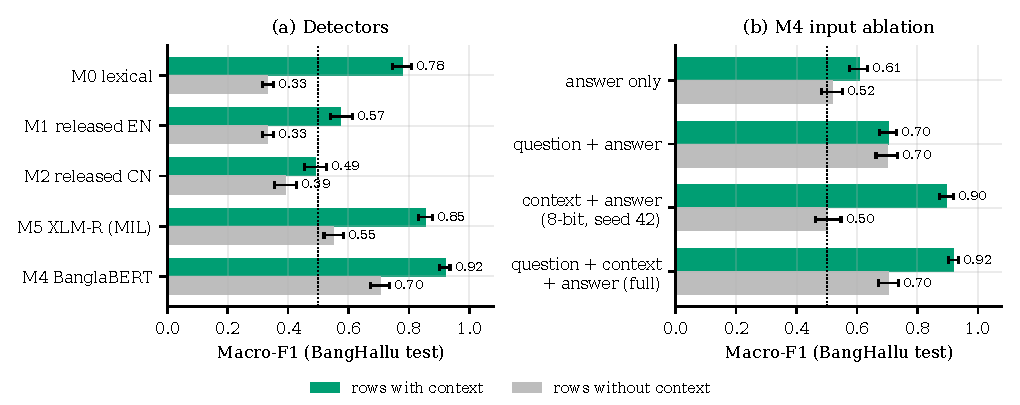
\includegraphics[width=\linewidth]{figures/fig_context_split.pdf}
\caption{Context availability and input ablation (post hoc). (a)~Macro-F1 of the detectors on BangHallu test rows with and without context (95\% bootstrap intervals). (b)~The same split for M4 trained on reduced input: without context, the full model and the question-and-answer model coincide. Dotted line: chance.}
\Description{Two horizontal bar charts of Macro-F1 on test rows with and without a context passage, with confidence intervals. Left: five detectors; every detector is near or below chance without context except the fine-tuned models, and BanglaBERT-large scores 0.92 with context and 0.70 without. Right: BanglaBERT-large trained on reduced input; the question-and-answer model scores 0.70 on both subsets and the full model 0.92 and 0.70.}
\label{fig:context}
\end{figure}

\subsection{External evaluation on Olikbochon (RQ4)}\label{sec:olik}
Table~\ref{tab:olik} reports the frozen detectors on Olikbochon. BanglaBERT-large (M4) reaches 0.698 $\pm$ 0.032 on all 299 rows, 0.134 below its BangHallu score; after removing the 30 rows that have an exact or near duplicate in the training set (post hoc), it reaches 0.684 $\pm$ 0.038 (CI $[0.636, 0.730]$), 0.148 below. Leakage accounts for 0.014 of the score and does not change the picture. The released detectors stay near chance (0.542 and 0.561, 0.544 and 0.546 after filtering) and below M0. The lexical baseline is close to M4 in F1: M4 exceeds M0 by 0.040 (paired CI $[-0.025, 0.103]$) on all rows and by 0.040 (CI $[-0.032, 0.109]$) on the clean rows, so the F1 advantage is not significant with 299 rows. The ranking quality is clearer: M4 has an AUROC of 0.782 (0.774 clean) against 0.629 (0.605) for M0. We did not re-tune thresholds on Olikbochon, so the F1 comparison also includes the cost of a threshold tuned on BangHallu. Olikbochon is small, 43.5\% of its rows have context, and we did not split it by context availability, so these numbers are a coarse external check.

\begin{table}[t]
\caption{External evaluation on Olikbochon with frozen BangHallu thresholds: M4 ranks better than the lexical baseline (AUROC) but its F1 advantage is not significant. ``Clean'' removes the 30 rows with an exact or near-duplicate in the training set (post hoc). Gap is the clean Olikbochon F1 minus the BangHallu F1.}
\label{tab:olik}
\small
\fit{\begin{tabular}{@{}lccccccc@{}}
\toprule
 & \multicolumn{2}{c}{Macro-F1} & & \multicolumn{2}{c}{AUROC} & BangHallu & Gap \\
\cmidrule(lr){2-3}\cmidrule(lr){5-6}
Model & all (299) & clean (269) & 95\% CI (clean) & all & clean & F1 & (clean) \\
\midrule
M0 & 0.658 & 0.644 & [0.586, 0.702] & 0.629 & 0.605 & 0.653 & $-0.009$ \\
M1 & 0.542 & 0.544 & [0.487, 0.603] & 0.602 & 0.592 & 0.533 & $+0.011$ \\
M2 & 0.561 & 0.546 & [0.486, 0.602] & 0.598 & 0.582 & 0.508 & $+0.038$ \\
M4 & 0.698 $\pm$ 0.032 & 0.684 $\pm$ 0.038 & [0.636, 0.730] & 0.782 & 0.774 & 0.832 & $-0.148$ \\
\bottomrule
\end{tabular}}
\end{table}

\subsection{Legal-domain shift (RQ4)}\label{sec:legal}
\paragraph{Setup.}
BanglaGovRAG and BD Legal QA supply 1,607 questions (971 Bengali, 635 English and one code-mixed in the retrieval evaluation) with reference answers but no hallucination labels. We index the 1,096 source documents as 1,219 chunks of 120 words with a stride of 100, and retrieve with BM25 \cite{robertson2009bm25} and multilingual-E5 \cite{wang2024e5} embeddings, fused by reciprocal rank fusion \cite{cormack2009rrf}. Retrieval is weak: Recall@1 is 0.228, Recall@5 0.409 and MRR 0.318 overall, and Bengali questions (Recall@1 0.185) are harder than English ones (0.291). To obtain labelled detection data, we pair each reference answer (label 0) with one synthetic perturbation (label 1): an entity swap (566 pairs), a negation (40), a changed number (9), or an unsupported addition (67), giving 1,364 examples. Evidence is either the gold passage or the top three retrieved chunks. This test is synthetic and its labels are not human-verified; it measures sensitivity to inserted errors, not the rate of natural legal hallucinations. M3 (XLM-R sequence classifier) and M4 (BanglaBERT-large) are the BangHallu-trained models applied without further training.

\paragraph{Detection.}
Table~\ref{tab:legal} and Figure~\ref{fig:legal} show that M4 is best but not good: Macro-F1 is 0.666 $\pm$ 0.140 with gold evidence and 0.571 $\pm$ 0.067 with retrieved evidence, with AUROC of 0.797 and 0.640. The large seed variance (0.140) means that individual M4 runs differ considerably in how well they transfer. The false-alarm rate of M4 is high (0.462 with gold evidence), and recall depends strongly on the perturbation type: 0.870 for entity swaps and 0.852 for number changes (nine examples), but 0.542 for negations and 0.582 for unsupported additions. M1 and M0 flag almost everything (false-alarm rates with gold evidence of 0.946 for M1 and 0.852 for M0), which gives high recall and an F1 below 0.46; M2 flags little (recall 0.323 for entity swaps, 0.125 for negations). The results for Bengali and English legal questions are similar (M4 0.657 and 0.680 with gold evidence). Retrieved evidence lowers F1 for M4 by 0.095, but weak retrieval confounds this: the detector sees the wrong passage for most questions.

\begin{table}[t]
\caption{Legal detection (reference answer vs.\ synthetic perturbation; 1,364 examples): M4 is best, with a high false-alarm rate and large seed variance. Recall is hallucination recall; FAR is the false-alarm rate on reference answers. Mean $\pm$ SD over seeds for M3 and M4.}
\label{tab:legal}
\small
\fit{\begin{tabular}{@{}lcccccccc@{}}
\toprule
 & \multicolumn{4}{c}{Gold evidence} & \multicolumn{4}{c}{Retrieved evidence} \\
\cmidrule(lr){2-5}\cmidrule(lr){6-9}
Model & F1 & Recall & FAR & AUROC & F1 & Recall & FAR & AUROC \\
\midrule
M0 & 0.452 & 0.918 & 0.852 & 0.472 & 0.387 & 0.908 & 0.922 & 0.464 \\
M1 & 0.370 & 0.925 & 0.946 & 0.595 & 0.408 & 0.815 & 0.864 & 0.574 \\
M2 & 0.546 & 0.330 & 0.185 & 0.555 & 0.597 & 0.474 & 0.267 & 0.562 \\
M3 & 0.492 $\pm$ 0.015 & 0.540 $\pm$ 0.146 & 0.538 $\pm$ 0.161 & 0.505 $\pm$ 0.007 & 0.453 $\pm$ 0.042 & 0.278 $\pm$ 0.197 & 0.287 $\pm$ 0.202 & 0.495 $\pm$ 0.002 \\
M4 & 0.666 $\pm$ 0.140 & 0.823 $\pm$ 0.064 & 0.462 $\pm$ 0.247 & 0.797 $\pm$ 0.085 & 0.571 $\pm$ 0.067 & 0.669 $\pm$ 0.093 & 0.511 $\pm$ 0.160 & 0.640 $\pm$ 0.047 \\
\bottomrule
\end{tabular}}
\end{table}

\begin{figure}[t]
\centering
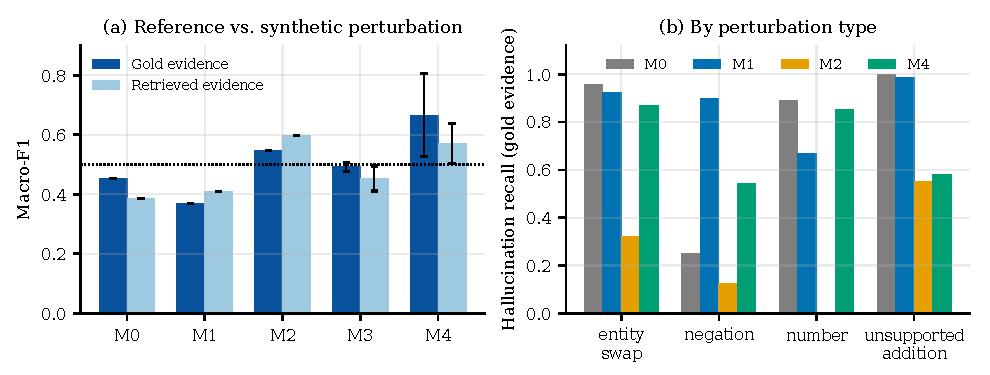
\includegraphics[width=\linewidth]{figures/fig_legal.pdf}
\caption{Legal stress test. (a)~Macro-F1 with gold and retrieved evidence (error bars: SD over seeds; none for deterministic models): retrieved evidence lowers F1 for M0, M3 and M4 and raises it for M1 and M2. (b)~Hallucination recall by perturbation type with gold evidence (only nine ``number'' examples): recall varies strongly by type.}
\Description{Two-panel bar chart. Left: Macro-F1 on the synthetic legal detection task with gold and retrieved evidence for five models; BanglaBERT-large is highest at 0.67 and 0.57. Right: hallucination recall by perturbation type for four models; recall differs strongly across entity swaps, negations, number changes and unsupported additions, and negations are the hardest type for most models.}
\label{fig:legal}
\end{figure}

\paragraph{Answerability.}
We also removed the gold document and asked whether a detector flags the answer as unsupported (682 examples). The accuracy of M0 (0.988) and M1 (0.887) is an artefact of flagging nearly everything, as the false-alarm rates above show; M4 flags 0.539 $\pm$ 0.194 of such answers and M2 0.260. A refusal rule based on retriever similarity does not help either: at the best single threshold ($\theta=0.844$) it refuses 83.2\% of out-of-corpus questions but also 73.2\% of answerable ones (balanced accuracy 0.550). Neither detector scores nor retrieval similarity currently provide a reliable answerability signal for Bengali legal questions.

\subsection{Calibration, selective prediction and cost (RQ5)}\label{sec:calib}
The fine-tuned models are overconfident (Table~\ref{tab:calib}). The ECE of BanglaBERT-large (M4) is 0.117 on average and that of the XLM-R token detector (M5) 0.071. Temperature scaling \cite{guo2017calibration} fitted on the development set (post hoc; $T\approx 2.5$ for M4 and 1.7 for M5) reduces ECE to 0.085 and 0.038, negative log-likelihood from 0.511 to 0.363 for M4, and the Brier score from 0.136 to 0.114; because the threshold is mapped through the same monotone transform, F1 is unchanged. Residual ECE for M4 is still 0.085, so temperature scaling improves, but does not repair, its calibration. The dev-tuned thresholds of M4 vary widely across seeds (0.175, 0.575, 0.792), but the F1 at an untuned 0.5 threshold (0.823, 0.837, 0.829) is within 0.010 of the tuned values (0.833, 0.838, 0.824), so the variation reflects a flat F1 curve and not instability in ranking. For selective prediction, the AURC of M4 is 0.046, against 0.466 for M1, 0.486 for M2 and 0.451 for M3, whose risk at every coverage is near that of random guessing. Abstaining on the least confident predictions therefore pays off for M4 but not for the others.

\begin{table}[t]
\caption{Temperature scaling (post hoc; mean over three seeds, fitted on the development set, evaluated on test): calibration improves but M4 remains overconfident. Arrows go from before to after scaling. F1 ($\tau^*$) is unchanged by scaling; F1 (0.5) uses an untuned threshold.}
\label{tab:calib}
\small
\fit{\begin{tabular}{@{}lccccccc@{}}
\toprule
Model & $T$ & ECE & NLL & Brier & F1 ($\tau^*$) & F1 (0.5) \\
\midrule
M4 BanglaBERT-large & 2.54 & 0.117 $\rightarrow$ 0.085 & 0.511 $\rightarrow$ 0.363 & 0.136 $\rightarrow$ 0.114 & 0.832 & 0.830 \\
M5 XLM-R (MIL) & 1.66 & 0.071 $\rightarrow$ 0.038 & 0.512 $\rightarrow$ 0.475 & 0.168 $\rightarrow$ 0.161 & 0.730 & 0.724 \\
\bottomrule
\end{tabular}}
\end{table}

Table~\ref{tab:effic} lists cost. The lexical baseline takes 0.09~ms per example. M4 takes 8.8~ms and 784~MB of peak GPU memory for 0.832 Macro-F1; the XLM-R token detector takes 4.1~ms and 575~MB for 0.730. The 4-bit 3B verifier needs 106~ms and 2.9~GB and reaches 0.705 on its 600-example subset, so it is both slower and, in this setting, less accurate than the fine-tuned encoders; because its subset differs from the full test set, this comparison is indicative only.

\begin{table}[t]
\caption{Accuracy and cost on BangHallu test: the fine-tuned encoders are both more accurate and faster than the 4-bit LLM verifier. M6 is evaluated on a class-stratified subset of 600 examples; all others on the full 1,228.}
\label{tab:effic}
\small
\fit{\begin{tabular}{@{}lrrrr@{}}
\toprule
Model & Macro-F1 & Latency (ms/ex) & Peak VRAM (MB) & $n$ \\
\midrule
M0 lexical & 0.653 & 0.09 & -- (CPU) & 1,228 \\
M1 English LettuceDetect & 0.533 & 12.09 & 588 & 1,228 \\
M2 EuroBERT LettuceDetect & 0.508 & 7.10 & 675 & 1,228 \\
M3 XLM-R (collapsed) & 0.502 & 1.43 & 653 & 1,228 \\
M4 BanglaBERT-large & 0.832 & 8.75 & 784 & 1,228 \\
M5 XLM-R (MIL) & 0.730 & 4.13 & 575 & 1,228 \\
M6 Qwen2.5-3B, 4-bit (zero-shot) & 0.705 & 106.45 & 2,902 & 600 \\
\bottomrule
\end{tabular}}
\end{table}

\subsection{Error analysis}\label{sec:errors}
We used a rule-based tagger to assign each error to one of ten categories (numeric or date mismatch, entity substitution, negation, unsupported addition, contradiction, surface variation, truncation, script mismatch, digit variant, legal reference). To check it, we drew 100 BangHallu errors on rows with context, stratified by the tagger's category, and labelled them blind to the tagger output. The labels were drafted by an LLM annotator (Claude) and then reviewed row by row by the authors, with the tagger's categories hidden; the authors accepted all 100 without changes. Agreement with the tagger was 47.0\% (Cohen's $\kappa=0.345$; 54.0\% and $\kappa=0.340$ at the level of five coarse buckets), which is below the 0.6 we had set as the bar for relying on the tagger. Its precision is acceptable for surface-form false alarms (0.81) and numeric mismatches (0.68) and poor for entity substitution (0.20) and contradiction (0.09); it never assigned negation, although six of the 100 sampled errors were negations. The category ``contradiction'' acts as a catch-all for number and entity errors.

We therefore do not report the tagger's raw counts. Table~\ref{tab:tax} reports coarse bucket shares of each model's with-context errors after correcting the tagger's counts with the confusion matrix between tagger and reviewed labels (resampling the labelled rows within each tagger stratum, 2,000 times, for the intervals). Factual-detail errors (numbers, dates, entities) are the largest category for every model (39--52\%), logical errors are a minority (11--20\%) and surface-form false alarms are 24--36\%. The raw tagger had attributed 61\% of the lexical baseline's (M0) errors and 29\% of the XLM-R token detector's (M5) to logical errors; the corrected shares are 13\% and 11\%. The correction assumes that the tagger confuses categories in the same way for all models, and the strata for tagger categories 4, 8, 9 and 10 contain one to three sampled rows each, so the intervals understate the uncertainty for them. Errors on rows without context (bottom of the table) cannot be categorised from the evidence.

\begin{table}[t]
\caption{Corrected shares of with-context errors by coarse bucket (95\% bootstrap interval in brackets): factual-detail errors dominate for every model. The last two rows give the number of errors on rows with and without context.}
\label{tab:tax}
\small
\fit{\begin{tabular}{@{}lccccc@{}}
\toprule
Error bucket & M0 & M1 & M2 & M4 & M5 \\
\midrule
Factual detail & 52\% [41, 64] & 40\% [32, 48] & 45\% [36, 53] & 41\% [26, 52] & 39\% [32, 45] \\
Logical & 13\% [3, 24] & 15\% [9, 21] & 18\% [12, 25] & 20\% [10, 34] & 11\% [6, 16] \\
Extrinsic content & 8\% [4, 12] & 13\% [7, 20] & 12\% [7, 19] & 10\% [5, 15] & 13\% [7, 20] \\
Surface / form & 25\% [20, 32] & 31\% [25, 36] & 24\% [19, 28] & 28\% [24, 33] & 36\% [29, 42] \\
Input processing & 1\% [0, 3] & 1\% [0, 3] & 1\% [0, 3] & 1\% [0, 3] & 1\% [0, 4] \\
\midrule
With-context errors ($n$) & 158 & 303 & 351 & 53 & 102 \\
Without-context errors ($n$) & 255 & 255 & 250 & 152 & 223 \\
\bottomrule
\end{tabular}}
\end{table}

\section{Discussion}\label{sec:discussion}
\paragraph{What the results show.}
The two released detectors fail on Bengali even when the evidence is present, and the failure is not explained by truncation. The tokenizer audit is consistent with a fragmentation account, but it is correlational. A Bengali-pretrained encoder recovers most of the gap with a few hundred labelled examples, which agrees with the finding of \citet{datta2026lowresource} that in-language supervision is what makes detectors work in a target language, and with the lower detection quality reported for other lower-resource languages \cite{ralethe2026multihallsa,abdaljalil2026halluverse}. That the same XLM-R backbone trains with a MIL token head but not with a sequence head in our setup suggests that, for lower-resource languages, the training formulation can matter as much as the choice of encoder; we have not identified why.

\paragraph{Implications for benchmarks.}
The BangHallu authors already separate rows with and without a passage \cite{banghalluRepo}. Our ablation adds evidence about detectors: on evidence-free rows the best detector is indistinguishable from a model that never sees evidence, and detectors that compare the answer with the context collapse to a single class there. An aggregate BangHallu score therefore mixes two tasks, checking an answer against evidence and judging whether an answer is plausible for a question. We hypothesise, without having tested it, that the second task rewards parametric knowledge or regularities of how the incorrect answers were constructed, and that it penalises detectors that only read the context. The practical consequence does not depend on that hypothesis: our own headline number, 0.832, is an average of 0.921 and 0.705, and claims of ``hallucination detection'' on such benchmarks should state which rows they rest on.

\paragraph{Recommendations for practitioners.}
For a Bengali RAG guardrail, the data support four recommendations. (1)~Do not reuse the released English or Chinese detectors as they are; in our evaluation they did not beat the lexical baseline. (2)~Fine-tune a Bengali-pretrained encoder: 564 labelled examples gave BanglaBERT-large 93\% of its full-data score. (3)~Where Bengali-pretrained weights are unavailable, an XLM-R token detector with a MIL loss (0.730, against 0.653 for the lexical baseline) is a viable fallback, although it trails BanglaBERT-large by about 0.10. (4)~Report results separately for rows with and without evidence, and do not deploy a detector in a high-stakes domain such as law on the strength of an in-domain score: in our legal stress test the best detector's false-alarm rate was 0.462 with gold evidence.

\section{Limitations}\label{sec:validity}
\paragraph{Internal validity.}
The context split, the input ablation, the M3 diagnostic, the Olikbochon leakage filter and temperature scaling were added after inspecting the main results; we label them as post hoc and verified that they leave the original thresholds and predictions unchanged. The XLM-R failure is unexplained, and both XLM-R models use frozen embeddings because of the 8~GB budget, which may disadvantage them. The reference M4 runs used an optimizer chosen automatically by memory estimate, whereas the single-seed 8-bit ablation rows used 8-bit AdamW explicitly; we record the optimizer of the new runs (fused AdamW) but could not read it for the reference runs. The threshold of the released detectors is tuned on Bengali development data, which can only favour them.

\paragraph{External validity.}
The main claims rest on one Bengali benchmark and a 299-row external set; we did not split Olikbochon by context, and the effects reported here may differ on other data. BangHallu's question--answer pairs were constructed with LLM assistance \cite{banghalluRepo}, so its incorrect answers may not resemble the hallucinations of a particular deployed system. The legal detection task uses synthetic perturbations without human validation, retrieval is weak, and the dev-tuned M4 thresholds were not re-tuned for the legal domain. M6 is evaluated on 600 examples, and we compared only one small quantized LLM, so we cannot say how larger LLM judges compare. We did not record dataset commit hashes, and one repository has changed since we downloaded it.

\paragraph{Construct validity.}
We measure answer-level Macro-F1, not span-level detection. On rows without context, a hallucination label can only reflect factual correctness, so these rows measure a different construct from the rows with context. The tokenizer analysis is correlational; it cannot separate fertility from the lack of Bengali pretraining. The error-analysis labels were drafted by an LLM and reviewed by the authors rather than annotated independently, and there is no second annotator; they validate the tagger's coarse behaviour, not a gold standard.

\paragraph{Statistical validity.}
We use three seeds, and the intervals for multi-seed models describe test-set sampling, not variation over training sets. Holm correction covers the four primary comparisons only; other intervals are descriptive. Paired-comparison F1 values are computed from majority votes and differ from the seed means reported elsewhere. Some strata of the error-correction bootstrap contain one to three rows, so their intervals understate the uncertainty.

\section{Ethical Considerations and Broader Impact}\label{sec:ethics}
All data are publicly available, and we collected no personal data. The study involves no human participants, and the error labels were reviewed by the authors themselves, so no ethics approval was required. BangHallu's text derives from Bengali Wikipedia (CC BY-SA 4.0) and from exam question banks whose redistribution terms its authors list as unresolved \cite{banghalluRepo}; we therefore release identifiers and predictions, not BangHallu text. BD Legal QA releases its own contributions under CC BY 4.0, excluding the quoted statutory text \cite{bdlegalqaRepo}, and the RAGTruth repository is released under the MIT licence; we found no licence statement for BanglaGovRAG \cite{banglagovragRepo} or for the Olikbochon competition data \cite{olikbochonKaggle}, and we release no text from any of these datasets. The legal results are a methodological study on synthetic perturbations and should not be taken as evidence that any detector is reliable enough for legal advice; in a high-stakes domain a detector with a false-alarm rate of 0.46 or a recall of 0.54 for negations is not a safeguard on its own. Both figures are measured against synthetic perturbations; on natural legal text the true rates could differ in either direction. The authors declare no competing interests.

\section{Conclusion and Future Work}\label{sec:conclusion}
\textbf{RQ1:} the two released LettuceDetect checkpoints we tested, trained on English and Chinese data, do not transfer to Bengali: they score below the lexical baseline even on rows with evidence, and truncation does not explain the failure. \textbf{RQ2:} a Bengali-pretrained encoder fine-tuned on a few hundred examples closes most of the gap, and the training formulation matters: an XLM-R sequence classifier did not train under our recipes while a token-level variant did. \textbf{RQ3:} in a post hoc analysis, our best detector uses the context on rows that have it and reaches 0.921 there; on the 41.5\% of test rows without evidence it behaves like a question--answer plausibility model. \textbf{RQ4:} external and legal-domain performance is clearly lower, and we report it with its uncertainty. \textbf{RQ5:} the fine-tuned detectors are overconfident, temperature scaling improves but does not repair calibration, and on a 600-example subset they were faster and more accurate than the 4-bit LLM verifier we tested.

Future work should test whether unfreezing the embeddings lets the XLM-R sequence classifier train, evaluate detectors on other Bengali benchmarks such as BenHalluEval \cite{adib2026benhallueval} and on the hard subset defined by the BangHallu authors, replace the synthetic legal perturbations with human-verified hallucinations from deployed legal RAG systems, use more training seeds, and validate the error taxonomy with a second, independent annotator.

\section*{Data and Code Availability}
All datasets are public (Section~\ref{sec:datasets}). The notebooks, frozen thresholds, per-example predictions (identifiers and scores, without dataset text), tables and figures behind every number in this paper are available at \url{https://github.com/HippomasAKiB1/turtlers_proofbangla} and archived on Zenodo (release v1.0.0, \url{https://doi.org/10.5281/zenodo.24136778}), together with a file that maps each table and figure to its source file. The 100 reviewed error labels, the key that links them to the tagger output and the script that computes agreement and the corrected shares are included. The original run and the post hoc analyses are in separate output directories, and the post hoc notebook verifies that the original outputs are unchanged.

\begin{acks}
The authors thank the maintainers of the public datasets used in this study. This research received no specific grant from any funding agency in the public, commercial, or not-for-profit sectors. Use of generative AI: a large language model (Claude, Anthropic) was used to draft the error-type labels described in Section~\ref{sec:errors}, which the authors then reviewed, to assist with analysis code, and to edit the text. The authors reviewed all outputs and are responsible for the content; all reported numbers are generated from the saved result tables.
\end{acks}

\bibliographystyle{ACM-Reference-Format}
\bibliography{references}

\appendix
\section{Implementation Details}\label{app:impl}
Table~\ref{tab:impl} collects the settings described in Section~\ref{sec:method}.

\begin{table}[h]
\caption{Implementation details of the fine-tuned detectors and the evaluation.}
\label{tab:impl}
\small
\fit{\begin{tabular}{@{}>{\raggedright}p{3.6cm}>{\raggedright\arraybackslash}p{9.4cm}@{}}
\toprule
Setting & Value \tabularnewline
\midrule
Optimizer & AdamW, weight decay 0.01; fused or 8-bit AdamW chosen by memory estimate \tabularnewline
Schedule & linear, 10\% warm-up; gradient clipping 1.0 \tabularnewline
Batch & effective batch size 16 by gradient accumulation; bf16 autocast \tabularnewline
Maximum input length & 512 tokens (fine-tuned models); 4,096 tokens (M1, M2); context truncated, never the answer \tabularnewline
Learning rate, epochs: M4 & $1.5\times10^{-5}$; 5, 8, 10 epochs for 100\%, 25\%, 10\% of the training data \tabularnewline
Learning rate, epochs: M5 & $2\times10^{-5}$; 5 epochs \tabularnewline
Learning rate, epochs: M3 (original) & $3\times10^{-5}$; 8, 10, 12 epochs; no normalizer \tabularnewline
Early stopping & development AUROC, patience 4 epochs \tabularnewline
Seeds & 42, 1337, 2026; 10\% and 25\% subsets sampled in question groups \tabularnewline
Frozen parameters & word-embedding matrices of the XLM-R models (M3, M5) \tabularnewline
M6 & 4-bit NF4; threshold on a stratified 300-example dev subset; evaluated on a stratified 600-example test subset \tabularnewline
Threshold $\tau^*$ & maximizes Macro-F1 on BangHallu dev; frozen for all test, external and legal sets \tabularnewline
Intervals & 95\% percentile bootstrap, 1,000 resamples; error-share correction 2,000 resamples \tabularnewline
ECE & ten equal-width bins, top-label confidence \tabularnewline
Hardware & one NVIDIA RTX 4060, 8~GB \tabularnewline
\bottomrule
\end{tabular}
}
\end{table}

\end{document}
